\chapter{Uczenie maszynowe}
\label{cha:uczenieMaszynowe}

Istnieje wiele metod, jakimi można podejść do zagadnienia rozpoznawania mowy. Spośród dostępnych otwartych (ang. open-source) oprogramowań wyróżnia się biblioteka \textit{SpeechRecognition} \cite{speechrec}, która umożliwia korzystanie z kilku popularniejszych Interfejsów Programistycznych Aplikacji (ang. API - Application Programming Interface) do rozpoznawania głosowego, w tym Google Web Speech API \cite{webspeech}. 

%---------------------------------------------------------------------------

\section{Środowisko zdalne}
\label{sec:srodZdal}

Używając biblioteki \textit{SpeechRecognition} możliwe jest zarówno rozpoznawanie mowy na podstawie nagrania \ref{fig:record} oraz odczytu z mikrofonu \ref{fig:microphone}. Przykłady połączenia jej on-line z zewnętrznym API, gdzie jako dane wejściowe zostało użyte nagranie oraz wypowiedzenie tej samej kwestii "go forward", znajdują się poniżej.

Poprzez stworzenie nowej instancji \textit{Recognizer}, funkcja \textit{record} przekazuje swój odczyt z danych wejściowych do funkcji \textit{recognize google}, która używając Google API \cite{webspeech} rozpoznaje mowę.

\begin{lstlisting}[language=Python]
def file_recognition(file):
    r = sr.Recognizer()
    with sr.AudioFile(file) as source:
        audio_data = r.record(source)
        query = r.recognize_google(audio_data, language='en-US')
\end{lstlisting}

\begin{center}
    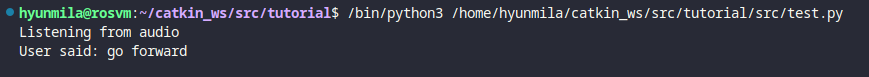
\includegraphics[width=12cm]{files/record.png}
    \captionof{figure}{Wynik funkcji służącej do odczytywania dźwięku z pliku audio.}
    \label{fig:record}
\end{center}

Analogicznie do znajdującej się powyżej, została napisana funkcja odczytująca dane z mikrofonu przy użyciu funkcji \textit{listen} przekazującej wynik do rozpoznania przez Google API \cite{webspeech}.

\begin{lstlisting}[language=Python]
def microphone_recognition():
    r = sr.Recognizer()
    with sr.Microphone() as mic:
        r.adjust_for_ambient_noise(mic)
        audio_data = r.listen(mic, timeout=5)
        query = r.recognize_google(audio_data, language='en-US')
\end{lstlisting}

\begin{center}
    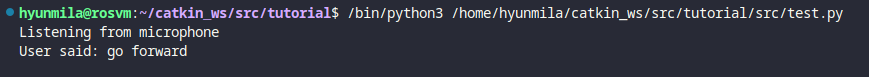
\includegraphics[width=12cm]{files/microphon1.png}
    \captionof{figure}{Wynik funkcji służącej do odczytywania dźwięku z mikrofonu}
    \label{fig:microphone}
\end{center}

Jak można zauważyć na podstawie wyników obu funkcji (\ref{fig:record}, \ref{fig:microphone}), otrzymany został z góry oczekiwany poprawny rezultat rozpoznania mowy. Jednak pomimo swojej wszechstronności zastosowań, biblioteka ta posiada istotne ograniczenia. Używanie któregokolwiek z interfejsów do rozpoznawania mowy wiąże się z potrzebą dostępu do stałego łącza internetowego i posiadania odpowiedniego klucza API. Jedynie dla Google Web Speech API jest on wbudowany, co nie zmienia faktu, że i ta funkcjonalność ma nałożone ograniczenie. Jako zaimplementowana tylko do przeprowadzania testów, w dowolnej chwili może zostać wycofana przez właściciela - Google - co czyni ją nieaplikowalną do celów produkcyjnych. Ponad to, ilość zapytań pod dany klucz API, nawet dla klucza prywatnego, jest odgórnie limitowana, co znacznie utrudnia zastosowanie którejkolwiek z metod poza środowiskiem testowym.

%---------------------------------------------------------------------------

\section{Środowisko lokalne}
\label{sec:srodLocal}

Innym podejściem do rozpoznawania mowy jest wykorzystanie istniejącego lub zbudowanie własnego modelu lokalnie. Istotą każdego algorytmu wykorzystującego uczenie maszynowe są dane, których użyto do jego wytrenowania. Zarówno dla zadania generowania tekstu, klasyfikacji obrazów czy właśnie rozpoznawania mowy, bez podania modelowi odpowiedniego rodzaju danych, nie jest możliwe osiągnięcie rzetelnego rezultatu. 

Głównym z problemów w kwestii dostępności danych do treningu jest różnica pomiędzy ilością danych opisanych etykietami (ang. labelled data), a nieopisanych (ang. unlabelled data). Ich proporcje są zazwyczaj bardzo nierówne - do uczenia na bazie danych audio istnieją tysiące godzin nagrań bez etykiet, w trakcie kiedy tych opisanych etykietami jest często setki razy mniej. 

Jak wspomniano w \ref{subsec:symbolic} język jest rzeczą płynną, ciągle się zmieniającą w zależności od upływu czasu, szerokości i długości geograficznej czy pochodzenia. Dwie osoby mówiące tym samym językiem mogą z perspektywy technicznej używać go zupełnie inaczej modulując tonację, akcent lub dialekt. Fakt ten sprawia, że zadanie znalezienia odpowiedniej ilości danych audio nagrań spełniających wszystkie kryteria każdego języka jest sporym wyzwaniem. Z tego powodu większość zestawów danych opiera się głównie na języku angielskim, używanym przez największą część populacji \cite{mostspoken}. 

Najprostszym rozwiązaniem jest użycie modelu już wytrenowanego, co umożliwia biblioteka \textit{Huggingface transformers} \cite{hf}. Zapewnia ona dostęp do wielu modeli uczenia maszynowego potrafiących rozpoznawać mowę, w tym do modelu \textit{Wav2Vec 2.0} \cite{baevski2020wav2vec} oraz \textit{Whisper} \cite{radford2022robust}.

%---------------------------------------------------------------------------

\subsection{Model Wav2Vec 2.0}
\label{subsec:wav2vec}

Model ten został najpierw wytrenowany na samych danych audio, a następnie dotrenowany za pomocą zestawu danych transkrybcji audio \textit{LibriSpeech} \cite{libri}. Ważną kwestią jest dobrany sposób trenowania, ponieważ autorzy postawili na użycie SSL, czyli samo-nadzorowanego uczenia (ang. self-supervised learning). Jest to metoda lekko odbiegająca od standardowych rozwiązań, bowiem łączy zarówno podejście nadzorowane jak i nienadzorowane. Modelowi przedstawiane są dane wejściowe bez etykiet oraz dane wyjściowe z etykietami. Bazując na tym, po podaniu mu kontekstu ma za zadanie przewidzieć wynik dla danych nieopisanych. 

Dane audio wchodzące do modelu są kodowane przez wielowarstwową konwolucyjną sieć neuronową (ang. CNN - Convolutional Neural Network). Podobnie jak w \textit{Maskowanym Modelowaniu Językowym} (ang. Masked Language Modelling) część danych, będąca uproszczonym modelem danych wejściowych, jest maskowana, a następnie podawana do sieci \textit{transformers}, która tworzy kontekstową reprezentację danych. Model jest następnie trenowany w zadaniu rozróżnienia prawdziwych danych od zakłóceń. 

Użyty w przykładowym algorytmie do rozpoznawania mowy model Wav2Vec to jego wersja dotrenowana na bazie \num{960} godzin audio o częstotliwości \num{16}kHz. Przy użyciu biblioteki \textit{torchaudio} plik audio jest odczytywany a następnie konwertowany do pożądanej przez model częstotliwości. Wektor audio jest następnie przekazywany do procesora modelu i wyciągana jest predykcja podawana do dekodera. Podany do rozpoznania ten sam plik audio, co w przykładzie \ref{sec:srodZdal} jest widoczny na Rys.\ref{fig:wav2vec}.

\begin{lstlisting}
def audio_reco(audio_path):
  speech, sr = torchaudio.load(audio_path)
  resampler = torchaudio.transforms.Resample(sr, 16000)
  speech = resampler(speech)
  input_features = wav2vec2_processor(speech.squeeze(), 
        return_tensors="pt", sampling_rate=16000)
  ...
  predicted_ids = torch.argmax(logits, dim=-1)
  transcription = wav2vec2_processor.batch_decode(predicted_ids)[0]
\end{lstlisting}

\begin{center}
    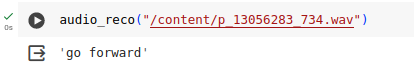
\includegraphics[width=12cm]{files/wav2vectest.png}
    \captionof{figure}{Wynik funkcji służącej do rozpoznawania mowy przy użyciu modelu Wav2Vec}
    \label{fig:wav2vec}
\end{center}

%---------------------------------------------------------------------------

\subsection{Model Whisper}
\label{subsec:whisper}

Drugi z wspomnianych wcześniej modeli rozszerza zakres zastosowań swojego poprzednika dzięki wytrenowaniu za pomocą zestawu danych \num{680,000} godzin zróżnicowanego audio w różnych językach do wykonywania nie tylko rozpoznawania mowy, ale też tłumaczenia, identyfikacji języka i detekcji aktywności głosowej. Dzięki innowatorskiemu podejściu autorów algorytmu, jest w stanie dostosowywać się on do zestawów danych obejmujących szeroki zakres, bez potrzeby dotrenowywania.

W poniższym przykładzie została użyta wersja \textit{medium} modelu, obsługująca wiele języków. Model tak samo jak w powyższym przypadku, przyjmuje dane audio i przetwarza je do częstotliwości \num{16}kHz. Następnie wyciągane są informacje o danych wejściowych i przekazywane do dekodera, który procesuje zadanie transkrybcji w języku angielskim. Otrzymany wynik rozpoznania pliku audio z przykładu \ref{sec:srodZdal} jest widoczny na Rys.\ref{fig:whisper}.

\begin{lstlisting}
def audio_reco(audio_path):
  ...
  forced_decoder_ids = whisper_processor.get_decoder_prompt_ids(
        language="english", task="transcribe")
  predicted_ids = whisper_model.generate(input_features, 
        forced_decoder_ids=forced_decoder_ids)
  transcription = whisper_processor.batch_decode(predicted_ids, 
        skip_special_tokens=True)[0]
\end{lstlisting}

\begin{center}
    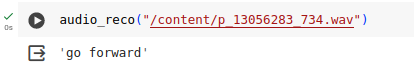
\includegraphics[width=12cm]{files/wav2vectest.png}
    \captionof{figure}{Wynik funkcji służącej do rozpoznawania mowy przy użyciu modelu Whisper}
    \label{fig:whisper}
\end{center}

%---------------------------------------------------------------------------

\section{Ewaluacja}
\label{sec:ewaluacja}

Ewaluacja algorytmów służących do rozpoznawania mowy polega na porównaniu predykcji wykonanej przez model do faktycznej transkrypcji i zapisaniu błędów popełnionych w trakcie zadania. Błędy te można podzielić na trzy kategorie:
\begin{itemize}
    \item zastępstwo (ang. substitution - S) - słowo zostało przetłumaczone w błędny sposób,
    \item dołożenie (ang. insertion - I) - zostało dodane dodatkowe, niewystępujące w nagraniu słowo,
    \item usunięcie (and. deletion - D) - słowo zostało pominięte.
\end{itemize}
Używaną do ewaluacji metryką jest \textit{WER - Word Error Rate}, która liczy błąd na poziomie każdego słowa. Dla audio, w którym wystąpiło N słów, \textit{WER} przedstawia się następująco:
\begin{equation}
    WER = \frac{S+I+D}{N}
\end{equation}

Do ewaluacji został wykorzystany zestaw danych \textit{edinburghcstr/ami} huggingface t\cite{dataset-eval}, składający się ze 100 godzin nagrań spotkań w języku angielskim. Przy użyciu biblioteki \textit{jiwer} \cite{jiwer}, przeprowadzono ewaluację powyższych algorytmów na podstawie zestawu danych \cite{dataset-eval}. Wyniki zostały przedstawione w tabeli \ref{tab:tab1}, gdzie wartość przy nazwie algorytmu jest wartością błędu każdego z nich w skali od 0 do 1.
\begin{table}[h]
    \centering
    \caption{Ewaluacja WER}
    \begin{tabular}{c|c|c}
        Wav2Vec & Whisper & SpeechRecognition  \\ 
        0.736557 & 0.713998 & 0.514967
    \end{tabular}
    \label{tab:tab1}
\end{table}
Oczywiście, wyniki te różnią się znacznie od podanych w pracach na temat wspomnianych powyżej algorytmów wartości zarówno z uwagi na fakt umieszczenia ich w lokalnym środowisku na maszynie bez jednostki obliczeniowej GPU, ale również jakości zestawu danych walidującego poprawność działania. Z uwagi na fakt prostoty w obsłudzie i najniższego współczynnika błędu, w dalszej części pracy jako algorytm będący podstawą działania panelu do sterowania głosowego zostało wybrane podejście zdalne i biblioteka \textit{SpeechRecognition} \cite{speechrec}.